\documentclass[color=usenames,dvipsnames]{beamer}\usepackage[]{graphicx}\usepackage[]{color}
%% maxwidth is the original width if it is less than linewidth
%% otherwise use linewidth (to make sure the graphics do not exceed the margin)
\makeatletter
\def\maxwidth{ %
  \ifdim\Gin@nat@width>\linewidth
    \linewidth
  \else
    \Gin@nat@width
  \fi
}
\makeatother

\definecolor{fgcolor}{rgb}{0, 0, 0}
\newcommand{\hlnum}[1]{\textcolor[rgb]{0.69,0.494,0}{#1}}%
\newcommand{\hlstr}[1]{\textcolor[rgb]{0.749,0.012,0.012}{#1}}%
\newcommand{\hlcom}[1]{\textcolor[rgb]{0.514,0.506,0.514}{\textit{#1}}}%
\newcommand{\hlopt}[1]{\textcolor[rgb]{0,0,0}{#1}}%
\newcommand{\hlstd}[1]{\textcolor[rgb]{0,0,0}{#1}}%
\newcommand{\hlkwa}[1]{\textcolor[rgb]{0,0,0}{\textbf{#1}}}%
\newcommand{\hlkwb}[1]{\textcolor[rgb]{0,0.341,0.682}{#1}}%
\newcommand{\hlkwc}[1]{\textcolor[rgb]{0,0,0}{\textbf{#1}}}%
\newcommand{\hlkwd}[1]{\textcolor[rgb]{0.004,0.004,0.506}{#1}}%
\let\hlipl\hlkwb

\usepackage{framed}
\makeatletter
\newenvironment{kframe}{%
 \def\at@end@of@kframe{}%
 \ifinner\ifhmode%
  \def\at@end@of@kframe{\end{minipage}}%
  \begin{minipage}{\columnwidth}%
 \fi\fi%
 \def\FrameCommand##1{\hskip\@totalleftmargin \hskip-\fboxsep
 \colorbox{shadecolor}{##1}\hskip-\fboxsep
     % There is no \\@totalrightmargin, so:
     \hskip-\linewidth \hskip-\@totalleftmargin \hskip\columnwidth}%
 \MakeFramed {\advance\hsize-\width
   \@totalleftmargin\z@ \linewidth\hsize
   \@setminipage}}%
 {\par\unskip\endMakeFramed%
 \at@end@of@kframe}
\makeatother

\definecolor{shadecolor}{rgb}{.97, .97, .97}
\definecolor{messagecolor}{rgb}{0, 0, 0}
\definecolor{warningcolor}{rgb}{1, 0, 1}
\definecolor{errorcolor}{rgb}{1, 0, 0}
\newenvironment{knitrout}{}{} % an empty environment to be redefined in TeX

\usepackage{alltt}
%\documentclass[color=usenames,dvipsnames,handout]{beamer}

%\usepackage[roman]{../../lab1}
\usepackage[sans]{../../lab1}
% \usepackage{Sweave}



\hypersetup{pdfpagemode=UseNone,pdfstartview=FitV}



\title{Lab 1 -- Introduction to {\bf R}}
\author{Richard Chandler and Bob Cooper}
\date{August 13 \& 14, 2018}

%\newcommand{\R}{{\bf R}}


%% Switching from Sweave to knitr
%\DefineVerbatimEnvironment{Sinput}{Verbatim}{fontshape=sl,formatcom=\color{red}}
%\DefineVerbatimEnvironment{Soutput}{Verbatim}{formatcom=\color{MidnightBlue}}
%\DefineVerbatimEnvironment{Scode}{Verbatim}{fontshape=sl}


% <<knitr-setup, include=FALSE>>=
% opts_hooks$set(comment=function(x) return("comment"=NA))
% ##knit_hooks$set(inline = function(x) {
% ##    if(!require(highr)) {
% ##        install.packages("highr")
% ##    }
% ##    if (is.numeric(x)) return(knitr:::format_sci(x, 'latex'))
% ##    highr:::hi_latex(x)
% ##})
% @













%% New command for inline code that isn't to be evaluated
\definecolor{inlinecolor}{rgb}{0.878, 0.918, 0.933}
\newcommand{\inr}[1]{\colorbox{inlinecolor}{\texttt{#1}}}
\IfFileExists{upquote.sty}{\usepackage{upquote}}{}
\begin{document}

% This would affect all code boxes. Not a good idea.
% \setlength\fboxsep{0pt}



\begin{frame}[plain]
  \LARGE
%  \maketitle
  {\centering
%  \textcolor{RoyalBlue}{\huge \bf Lab 1 -- Introduction to \R} \\
  {\huge \bf Lab 1 -- Introduction to \R} \\
  \vspace{0.9cm}
  
\includegraphics[width=0.4\textwidth]{figs/Rlogo} \\
  \vspace{0.5cm}
  August 13 \& 14, 2018 \\
  FANR 6750 \par
  \vfill
  \large
  Richard Chandler and Bob Cooper \\
  University of Georgia \\
  }
\end{frame}




\section{Why Use \R?}


\begin{frame}[plain]
  \frametitle{Today's Topics}
  \Large
  \only<1>{\tableofcontents}%[hideallsubsections]}
  \only<2 | handout:0>{\tableofcontents[currentsection]}%,hideallsubsections]}
\end{frame}



\begin{frame}
  \frametitle{Good and Not So Good Things About \R}
%  {\Large \textcolor{bb}{Good}}
  {\Large Good}
  \large
  \begin{itemize}%[<+->]
    \item<1-> Powerful platform for statistical analysis %Flexible %If you're going to use a stats program, might as well use one that does everything!
%    \item<1-> Many \inr{packages} \colorbox{BurntOrange}{written} for ecologists
    \item<1-> Many packages written for ecologists
    \item<1-> It's free
    \item<1-> Scripts save time
    \item<1-> \R~teaches you statistics
  \end{itemize}
  \vspace{0.5cm}
  \uncover<2->{
%  \pause
  {\Large Not so good??}}
  \begin{itemize}
    \item<2-> Steep learning curve
    \item<2-> Help pages written for people familiar with \R
    \item<2-> Developed by statisticians for statisticians
    \item<2-> Not as fast as some languages
  \end{itemize}
%  }
\end{frame}




%\begin{frame}
%  \frametitle{Not So Good Things About \R}
%\end{frame}




\section{Installing \R}





\begin{frame}
  \frametitle{Downloading \R}
  \begin{columns}
    \begin{column}{0.4\textwidth}
      \small
      \begin{itemize}
      \item Go to \url{www.r-project.org}
      \item Click on ``CRAN''
      \item Choose a mirror near you (there is one in TN)
      \end{itemize}
    \end{column}
    \begin{column}{0.6\textwidth}
      \fbox{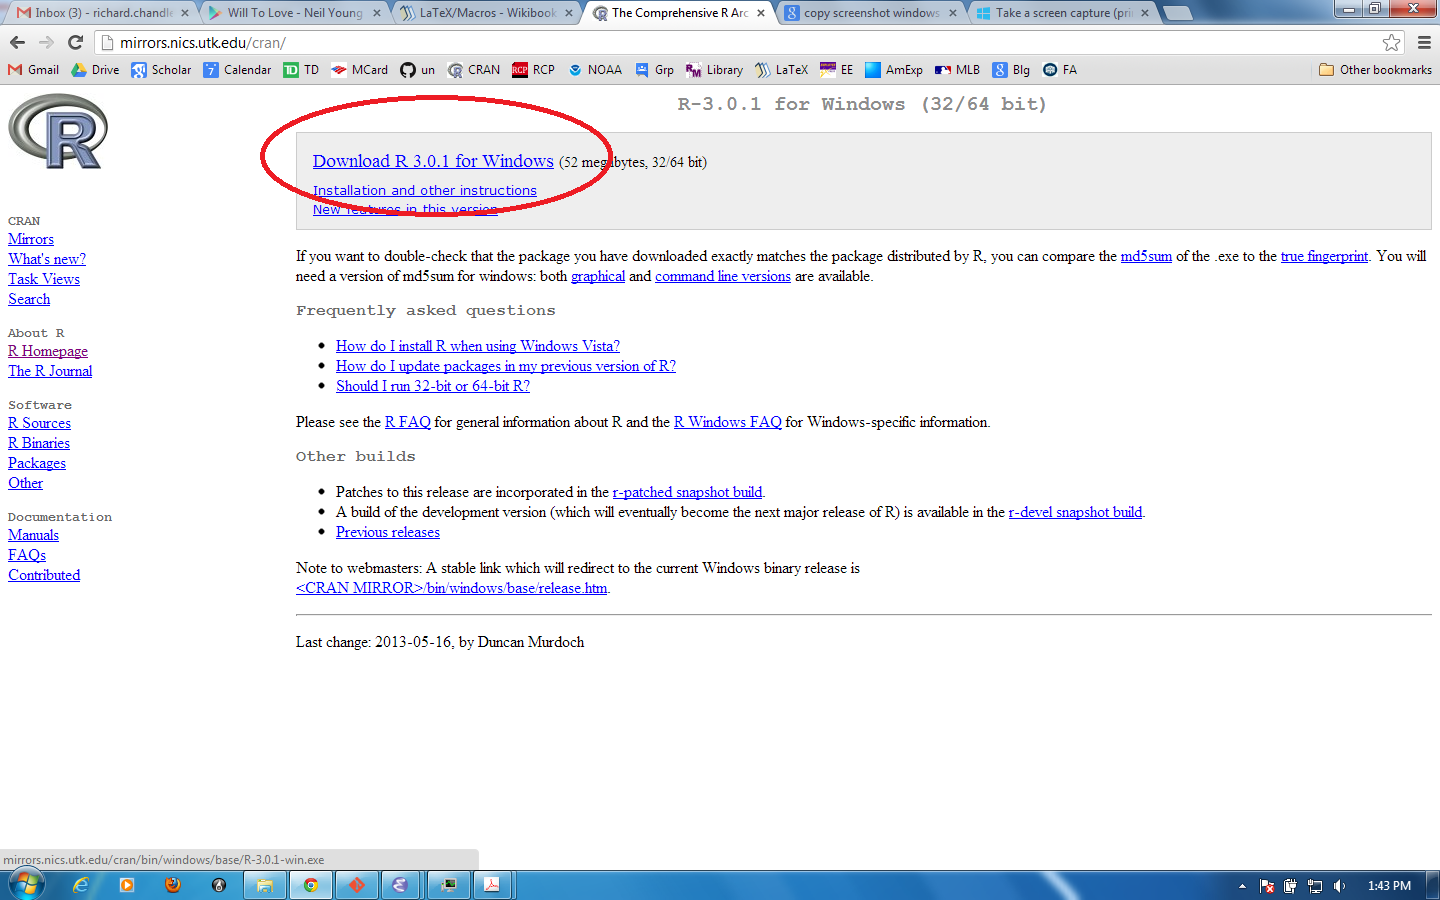
\includegraphics[width=\textwidth]{figs/download-R-win}} \par
      \fbox{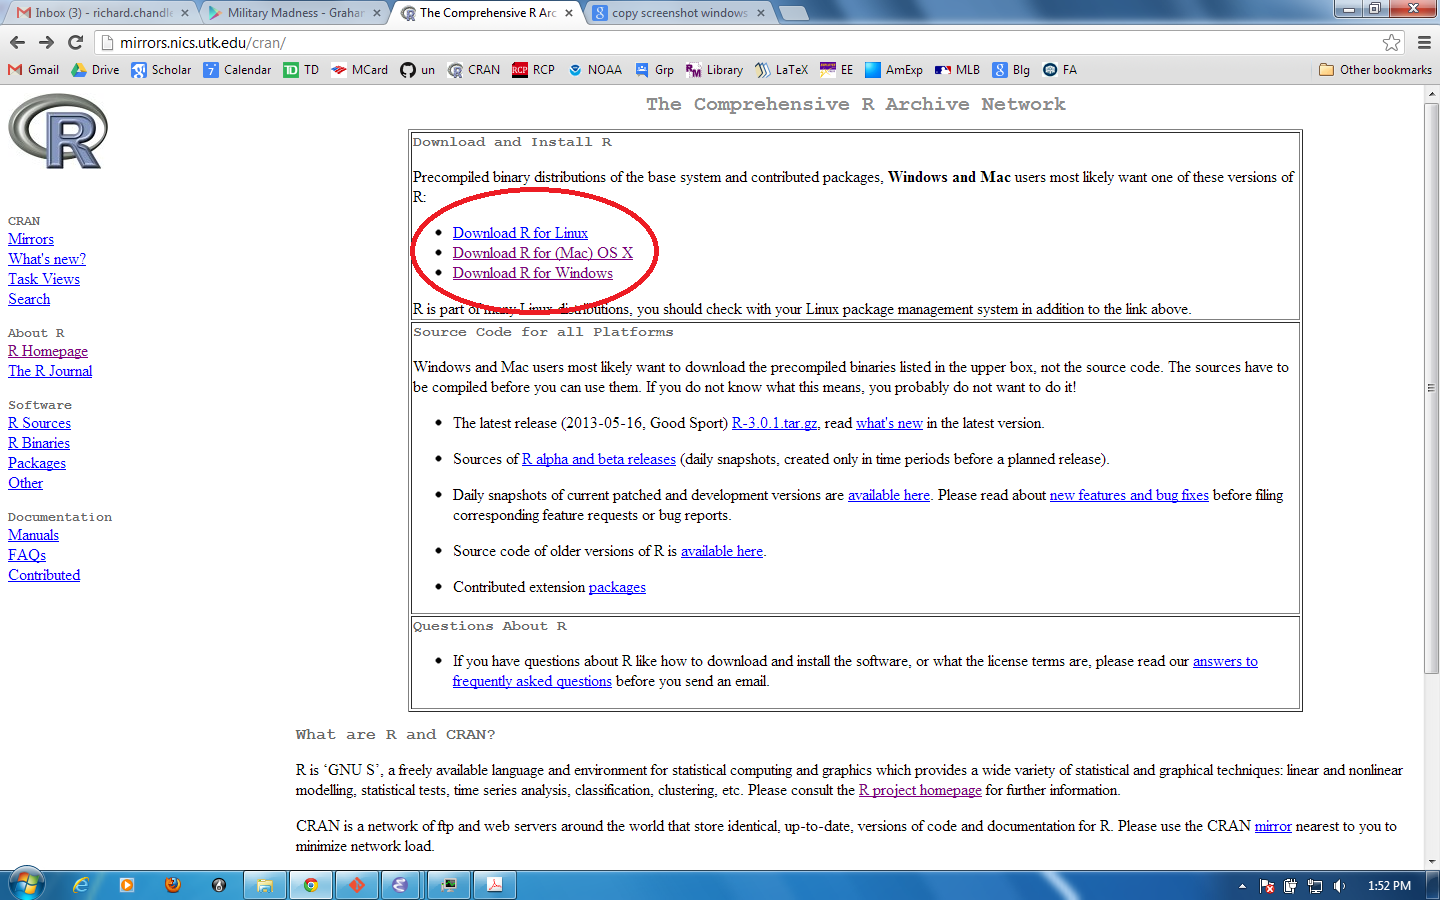
\includegraphics[width=\textwidth]{figs/download-R}}
    \end{column}
  \end{columns}
\end{frame}



\begin{frame}
  \frametitle{Using the \R~GUI}
  \R's ``Graphical User Interface'' is operating system specific. Here
  is how it looks under Windows.
  \begin{center}
    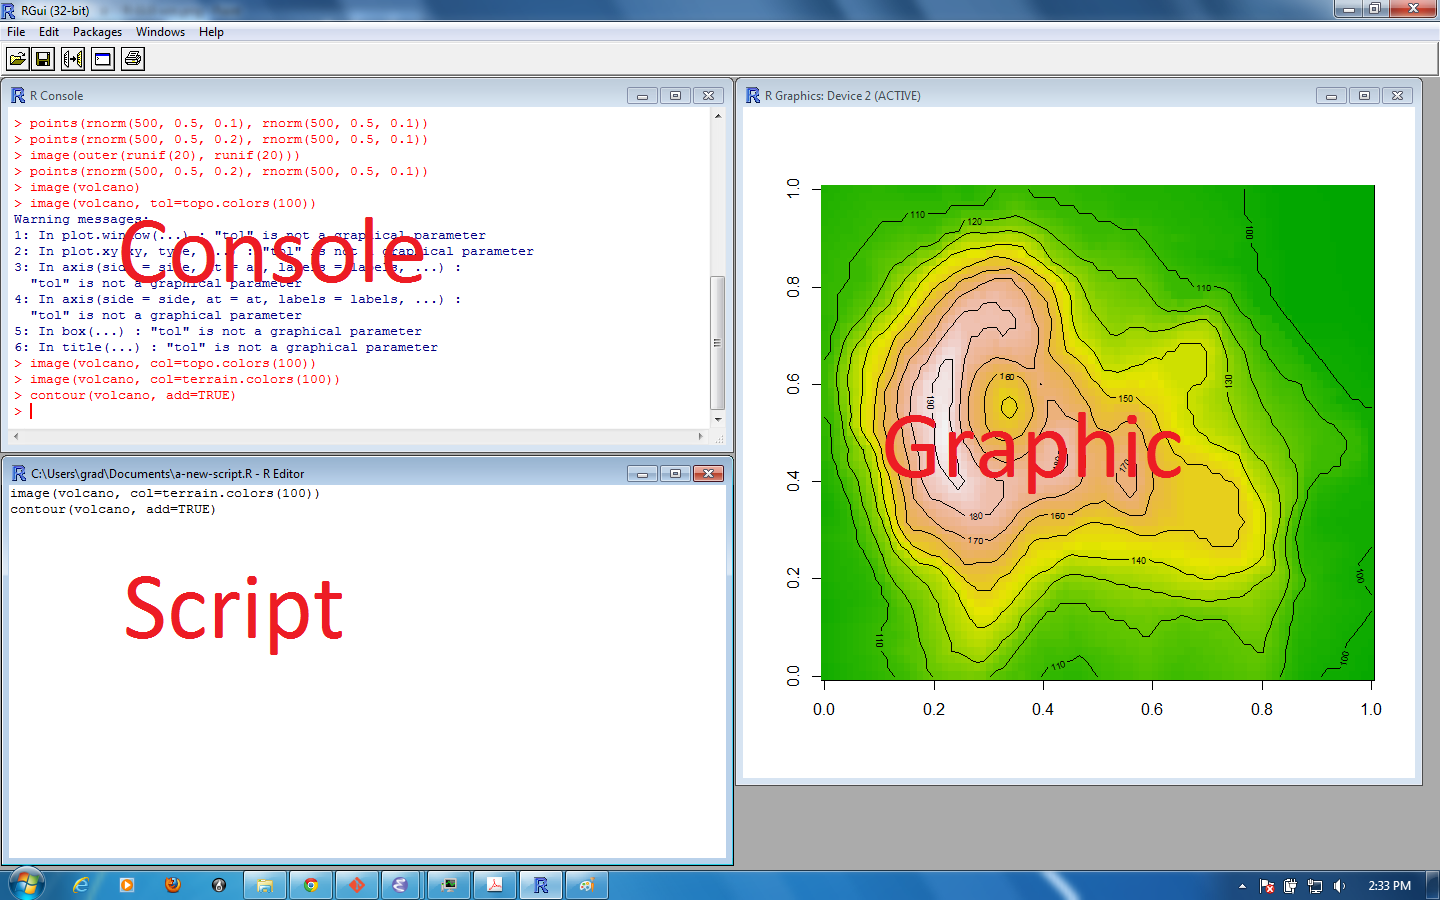
\includegraphics[width=\textwidth]{figs/R-GUI-win}
  \end{center}
\end{frame}



\begin{frame}
  \frametitle{Alternatives to the \R~Gui}
  \begin{columns}
    \small
    \begin{column}{0.6\textwidth}
      \centering
      Emacs and ESS \\ \tiny
      \url{http://vgoulet.act.ulaval.ca/en/emacs/} \par
      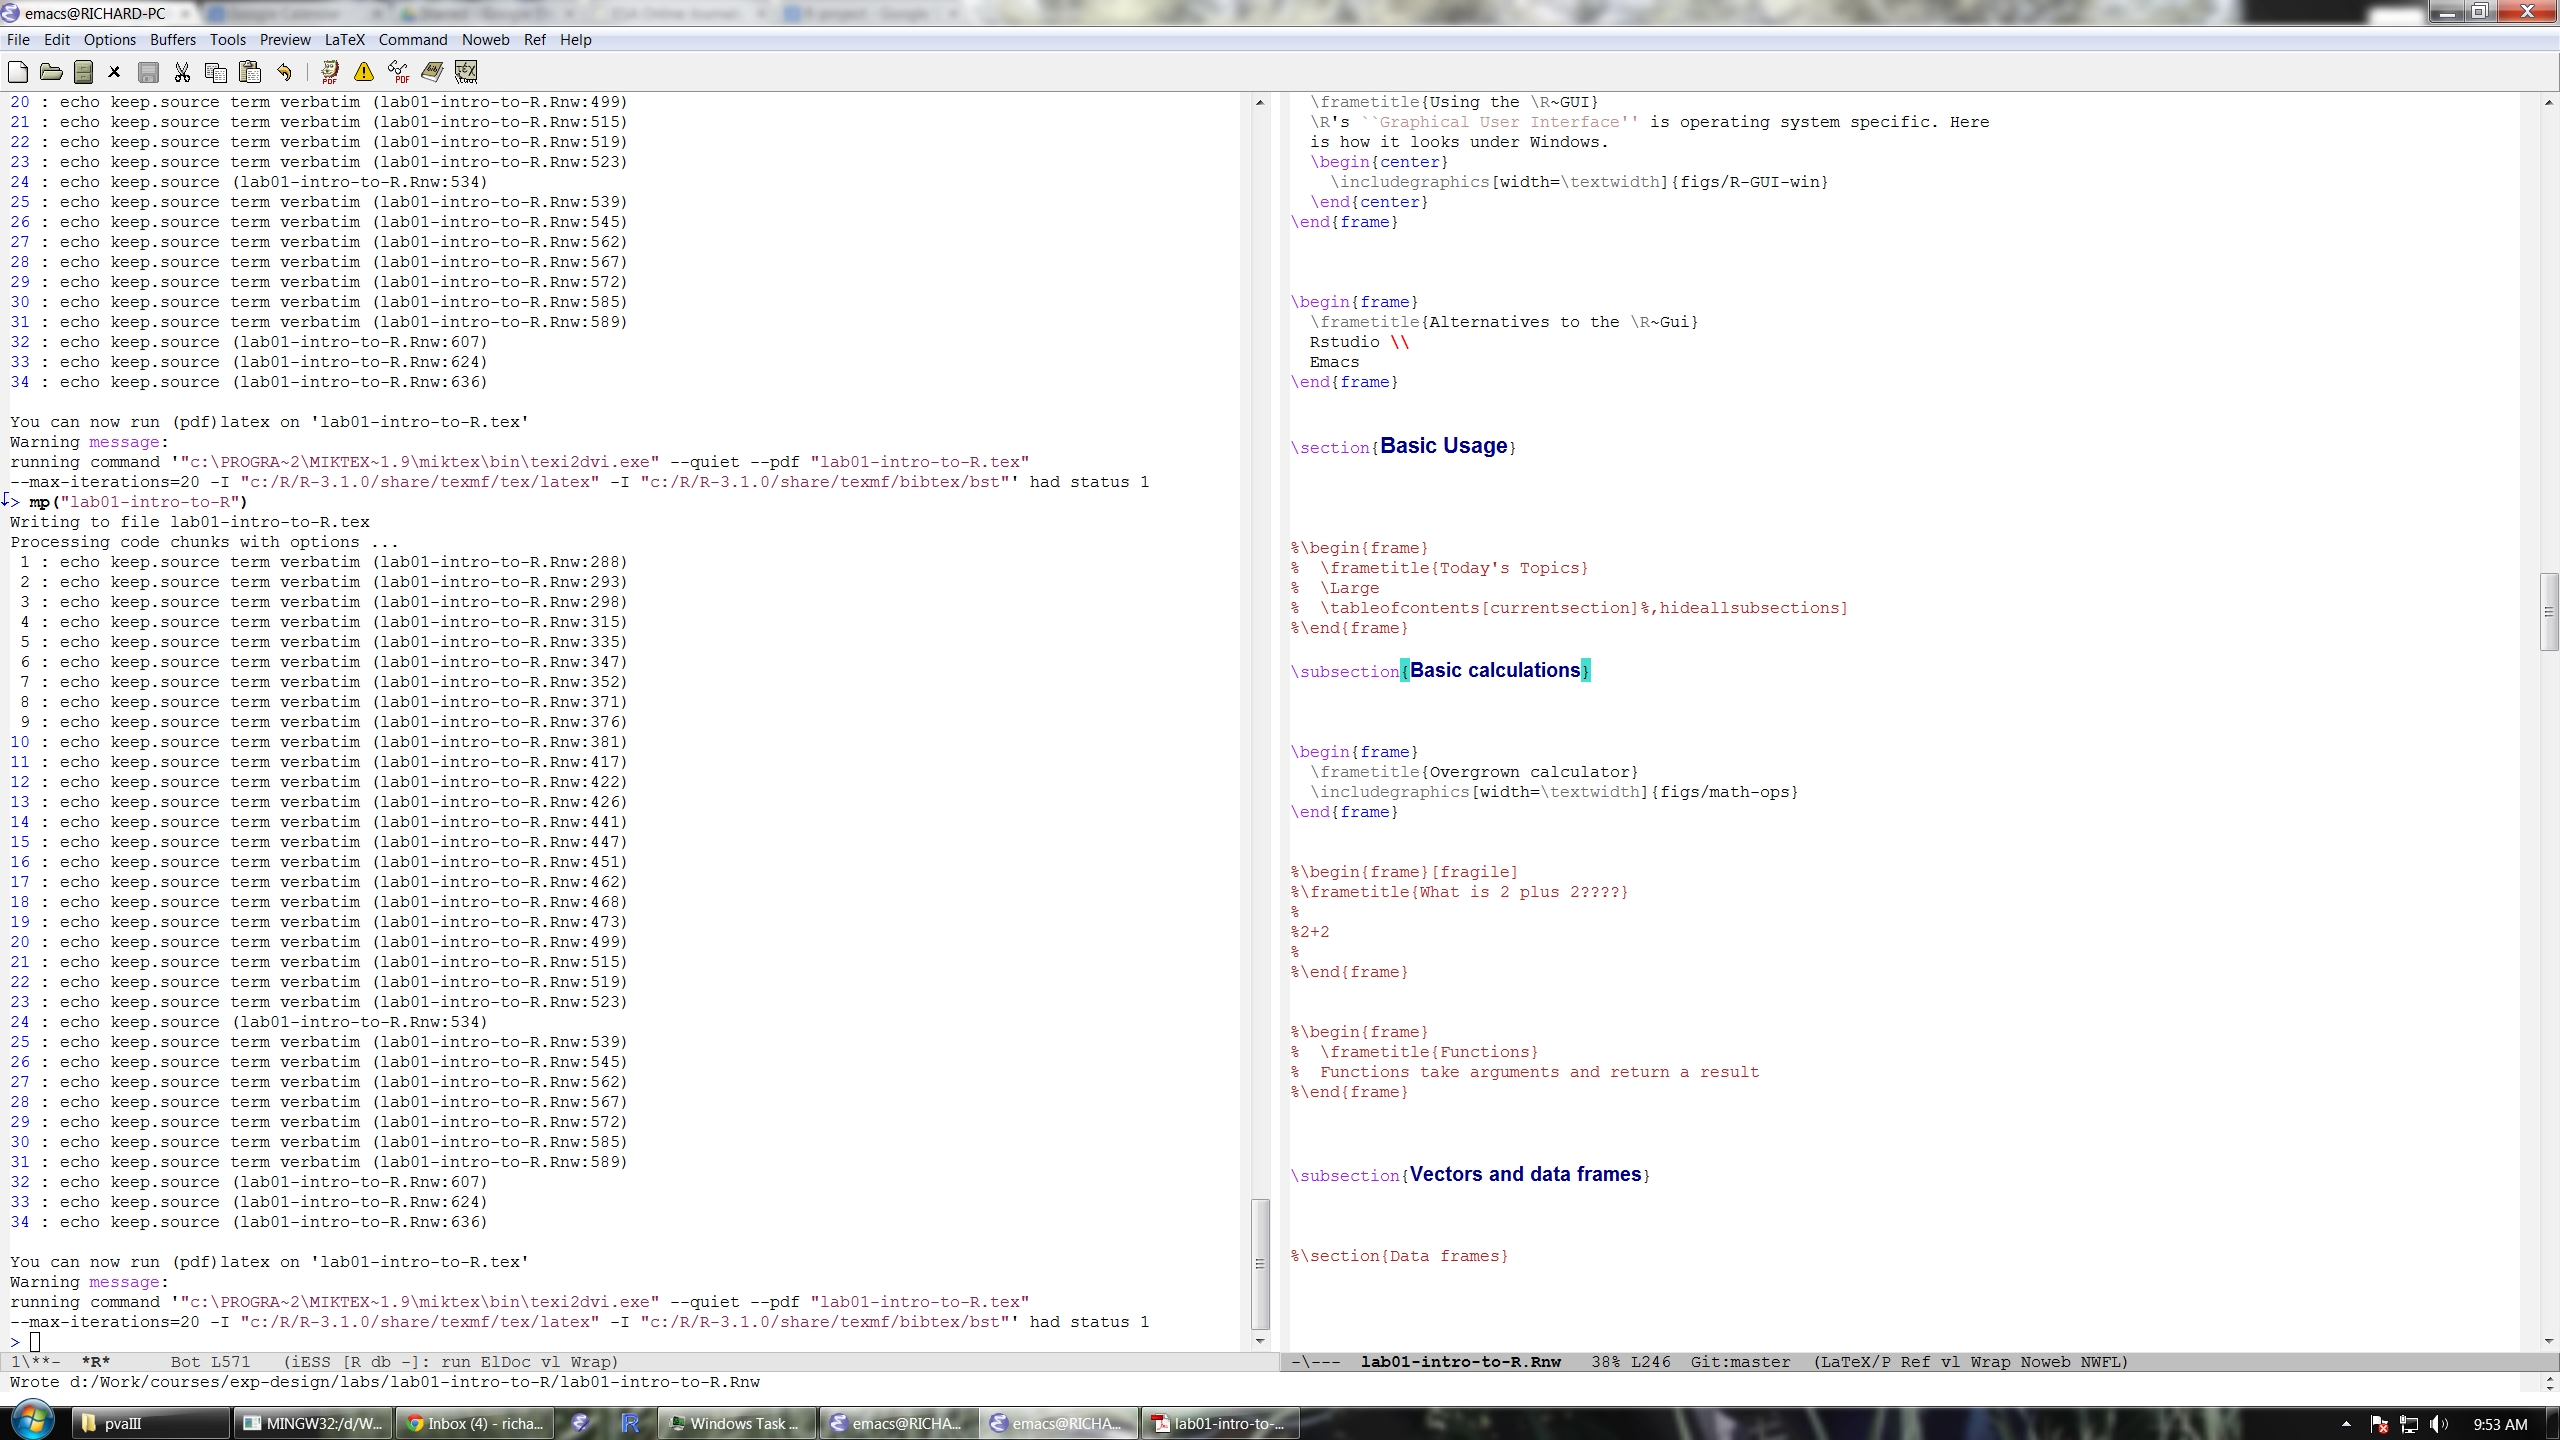
\includegraphics[width=\textwidth]{figs/emacs}
    \end{column}
    \begin{column}{0.4\textwidth}
      \centering
      RStudio \\
      \url{http://www.rstudio.com/} \par
      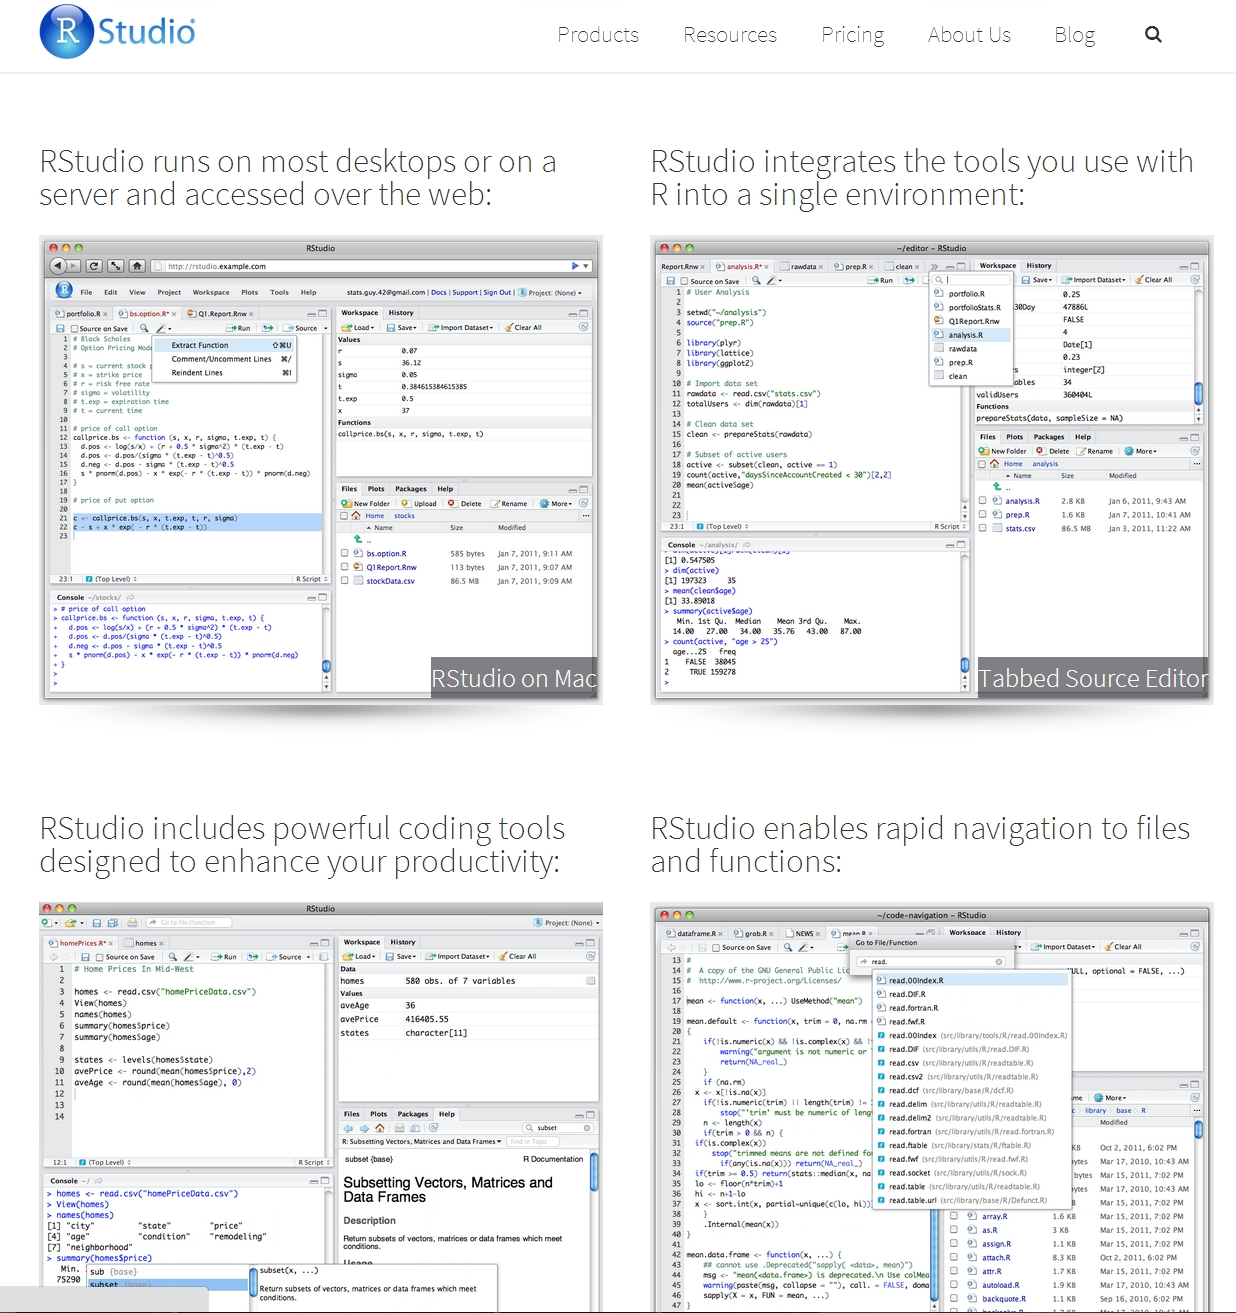
\includegraphics[width=\textwidth]{figs/Rstudio}
    \end{column}
  \end{columns}
%  \pause
  \small
  \vspace{0.5cm}
  You are encouraged to learn and use these programs, but we will not
  use them for instruction because we want to focus on \R~itself, not
  the interface.
\end{frame}


\section{Basic Usage}




%\begin{frame}
%  \frametitle{Today's Topics}
%  \Large
%  \tableofcontents[currentsection]%,hideallsubsections]
%\end{frame}

\subsection{Basic calculations}




\begin{frame}[fragile]
  \frametitle{How to read the code in the lab slides}
%  \small
  Anything in a shaded box like this one is \R~code:
\begin{knitrout}
\definecolor{shadecolor}{rgb}{0.878, 0.918, 0.933}\color{fgcolor}\begin{kframe}
\begin{alltt}
\hlnum{2}\hlopt{+}\hlnum{2}
\end{alltt}
\begin{verbatim}
## [1] 4
\end{verbatim}
\end{kframe}
\end{knitrout}
\pause %\vfill
  The line \inr{2+2} is \R~code (\alert{input}). You can copy
  and paste it into the console. Note that the command prompt (\verb+>+) is
  not shown.
\vfill
  The line \inr{\#\# [1] 4} is \alert{output}. Output is
  always indicated by two hash signs (\texttt{\#\#}). Anything after a
  \texttt{\#} is ignored by \R~at the command line.
\pause \vfill
  You can copy and paste the entire code box directly into your
  console, but it might be easier to work with the \R~script
  that accompanies the PDF: %. In this case, the script is called
  \texttt{lab-intro-to-R.R}.
\end{frame}






\begin{frame}[fragile]
  \frametitle{Overgrown calculator}
%  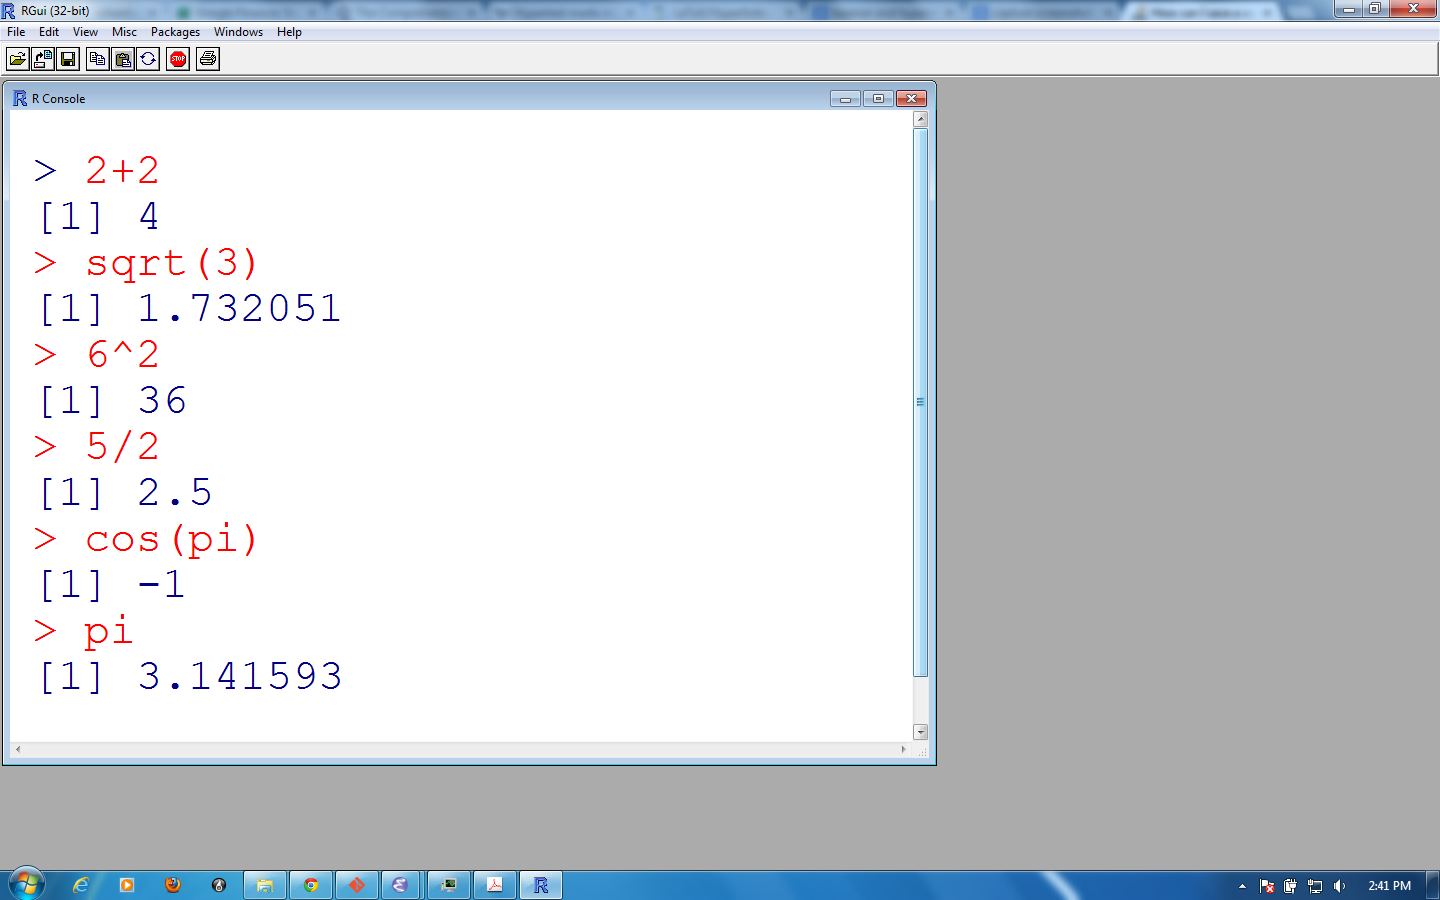
\includegraphics[width=\textwidth]{figs/math-ops}
  \small
%  Simple addition
%<<add, size='small'>>=
%2+2
%@
%\pause \vfill
  Square-root of 3
\begin{knitrout}\small
\definecolor{shadecolor}{rgb}{0.878, 0.918, 0.933}\color{fgcolor}\begin{kframe}
\begin{alltt}
\hlkwd{sqrt}\hlstd{(}\hlnum{3}\hlstd{)}
\end{alltt}
\begin{verbatim}
## [1] 1.732051
\end{verbatim}
\end{kframe}
\end{knitrout}
\pause \vfill
  6 squared
\begin{knitrout}\small
\definecolor{shadecolor}{rgb}{0.878, 0.918, 0.933}\color{fgcolor}\begin{kframe}
\begin{alltt}
\hlnum{6}\hlopt{^}\hlnum{2}
\end{alltt}
\begin{verbatim}
## [1] 36
\end{verbatim}
\end{kframe}
\end{knitrout}
\pause \vfill
  cosine of $\pi$
\begin{knitrout}\small
\definecolor{shadecolor}{rgb}{0.878, 0.918, 0.933}\color{fgcolor}\begin{kframe}
\begin{alltt}
\hlkwd{cos}\hlstd{(pi)}
\end{alltt}
\begin{verbatim}
## [1] -1
\end{verbatim}
\end{kframe}
\end{knitrout}
%<<pi>>=
%pi
%@
\end{frame}





%\section{Data frames}





\begin{frame}[fragile]
  \frametitle{Objects and assignment arrow}
%  {\Large Important things to know about objects:}
%  \begin{itemize}[<+->]
%    \item
      Everything in \R~is an object. We can create objects using the
      \inr{<-} assignment arrow.
      \pause \vfill
%    \item
      In this example, we assign the value 2 to the object \inr{y}:
\begin{knitrout}
\definecolor{shadecolor}{rgb}{0.878, 0.918, 0.933}\color{fgcolor}\begin{kframe}
\begin{alltt}
\hlstd{y} \hlkwb{<-} \hlnum{2}
\end{alltt}
\end{kframe}
\end{knitrout}
%\pause \vfill
%    \item The \colorbox{inlinecolor}{\texttt{<-}} arrow assigns the value y to the object \texttt{y}.
%    \item
%The \inr{<-} arrow assigns the value 2 to the object \inr{y}.
      \pause \vfill
%    \item
      You cannot have a space between \inr{<} and \inr{-}
      \pause \vfill
%    \item
      You can use \inr{=} instead of \inr{<-} but this can cause confusion
      \pause \vfill
%    \item
      Typing the name of an object returns its value:
\begin{knitrout}
\definecolor{shadecolor}{rgb}{0.878, 0.918, 0.933}\color{fgcolor}\begin{kframe}
\begin{alltt}
\hlstd{y}
\end{alltt}
\begin{verbatim}
## [1] 2
\end{verbatim}
\end{kframe}
\end{knitrout}
%  \end{itemize}
\end{frame}


\subsection{Vectors}


\begin{frame}[fragile]
  \frametitle{Vectors}
%  \begin{itemize}[<+->]
%    \item
We store data in objects so that they can be easily manipulated:
%  Notice how \inr{y} behaves just like the number 2:
\begin{knitrout}\small
\definecolor{shadecolor}{rgb}{0.878, 0.918, 0.933}\color{fgcolor}\begin{kframe}
\begin{alltt}
\hlstd{y}\hlopt{*}\hlnum{2}\hlopt{+}\hlnum{1}
\end{alltt}
\begin{verbatim}
## [1] 5
\end{verbatim}
\end{kframe}
\end{knitrout}
%    \item
\pause \vfill
Usually, we want more than one number in an object. In statistics, a
vector is simply a set of numbers that can be thought of as a row or
column of a matrix \\
%\item
\pause \vfill
The easiest way to create a vector is to use the \inr{c}
function to ``combine'' numbers:
\begin{knitrout}\small
\definecolor{shadecolor}{rgb}{0.878, 0.918, 0.933}\color{fgcolor}\begin{kframe}
\begin{alltt}
\hlstd{z} \hlkwb{<-} \hlkwd{c}\hlstd{(}\hlopt{-}\hlnum{1}\hlstd{,} \hlnum{9}\hlstd{,} \hlnum{33}\hlstd{,} \hlopt{-}\hlnum{4}\hlstd{)}
\hlstd{z}
\end{alltt}
\begin{verbatim}
## [1] -1  9 33 -4
\end{verbatim}
\end{kframe}
\end{knitrout}
%  \end{itemize}
\end{frame}



%% \begin{frame}[fragile]
%%   \frametitle{Vectors}
%% %  \begin{block}{Definition}
%% %  \Large
%%   \begin{itemize}
%% %    \item In statistics, a vector is a set of numbers
%%     \item The easiest way to create a vector is to use the \verb+c+
%%       function to ``combine'' numbers
%%   \end{itemize}
%% <<>>=
%% x <- c(1, 2, 3, 9, -100)
%% x
%% @
%% %  \end{block}
%% %  This code creates a vector of continuous numbers:

%% \end{frame}


%\begin{frame}
%  \frametitle{More about the assignment arrow}
%
%\end{frame}


\begin{frame}[fragile]
  \frametitle{Other useful ways of creating vectors}
%\begin{itemize}[<+->]
%  \item The easiest way to create a vector is to use the \verb+c+
%      function to ``combine'' numbers
%<<>>=
%x1 <- c(1, 2, 3, 9, -100)
%x1
%@
%  \item
A sequence of numbers
\begin{knitrout}\small
\definecolor{shadecolor}{rgb}{0.878, 0.918, 0.933}\color{fgcolor}\begin{kframe}
\begin{alltt}
\hlstd{x1} \hlkwb{<-} \hlnum{1}\hlopt{:}\hlnum{3} \hlcom{# Same as: x1 <- c(1, 2, 3)}
          \hlcom{# Note: anything after "#" is a comment}
\hlstd{x1}
\end{alltt}
\begin{verbatim}
## [1] 1 2 3
\end{verbatim}
\end{kframe}
\end{knitrout}
\pause \vfill
%\item
\inr{seq} is more general
%% <<>>=
%% x2 <- seq(from=1, to=3, by=1)
%% x2
%% @
%% \item[]
\begin{knitrout}\small
\definecolor{shadecolor}{rgb}{0.878, 0.918, 0.933}\color{fgcolor}\begin{kframe}
\begin{alltt}
\hlstd{x2} \hlkwb{<-} \hlkwd{seq}\hlstd{(}\hlkwc{from}\hlstd{=}\hlnum{1}\hlstd{,} \hlkwc{to}\hlstd{=}\hlnum{7}\hlstd{,} \hlkwc{by}\hlstd{=}\hlnum{2}\hlstd{)}
\hlstd{x2}
\end{alltt}
\begin{verbatim}
## [1] 1 3 5 7
\end{verbatim}
\end{kframe}
\end{knitrout}
%\item
\pause \vfill
Use \inr{rep} to repeat elements of a vector
\begin{knitrout}\small
\definecolor{shadecolor}{rgb}{0.878, 0.918, 0.933}\color{fgcolor}\begin{kframe}
\begin{alltt}
\hlkwd{rep}\hlstd{(x2,} \hlkwc{times}\hlstd{=}\hlnum{2}\hlstd{)}
\end{alltt}
\begin{verbatim}
## [1] 1 3 5 7 1 3 5 7
\end{verbatim}
\end{kframe}
\end{knitrout}
%\end{itemize}
\end{frame}



\begin{frame}[fragile]
  \frametitle{Help with a function}
\LARGE
These do the same thing
\begin{knitrout}
\definecolor{shadecolor}{rgb}{0.878, 0.918, 0.933}\color{fgcolor}\begin{kframe}
\begin{alltt}
\hlopt{?}\hlstd{rep}
\hlkwd{help}\hlstd{(rep)}
\end{alltt}
\end{kframe}
\end{knitrout}
\end{frame}




\begin{frame}[fragile]
  \frametitle{Types of vectors}
%  \begin{itemize}[<+->]
%  \item
  Numeric vectors are used for continuous variables
\begin{knitrout}\small
\definecolor{shadecolor}{rgb}{0.878, 0.918, 0.933}\color{fgcolor}\begin{kframe}
\begin{alltt}
\hlstd{y1} \hlkwb{<-} \hlkwd{c}\hlstd{(}\hlnum{2.1}\hlstd{,} \hlnum{3.5}\hlstd{,} \hlnum{99.0}\hlstd{)}
\hlkwd{class}\hlstd{(y1)}
\end{alltt}
\begin{verbatim}
## [1] "numeric"
\end{verbatim}
\end{kframe}
\end{knitrout}
%  \item
\pause \vfill
%  Names can be stored as character vectors
%<<y2-class, size='small'>>=
%y2 <- c("Treatment", "Control")
%class(y2)
%@
%  \item
%\pause \vfill
Factors can be used to store categorical variables: %character strings
\begin{knitrout}\small
\definecolor{shadecolor}{rgb}{0.878, 0.918, 0.933}\color{fgcolor}\begin{kframe}
\begin{alltt}
\hlstd{y2} \hlkwb{<-} \hlkwd{factor}\hlstd{(}\hlkwd{c}\hlstd{(}\hlstr{"Treatment"}\hlstd{,} \hlstr{"Control"}\hlstd{,} \hlstr{"Treatment"}\hlstd{))}
\hlstd{y2}
\end{alltt}
\begin{verbatim}
## [1] Treatment Control   Treatment
## Levels: Control Treatment
\end{verbatim}
\end{kframe}
\end{knitrout}
%  \end{itemize}
\end{frame}



\begin{frame}[fragile]
  \frametitle{Vectorized arithmetic}
  How could we calculate the body mass index (BMI = $\text{weight}/\text{height}^2$) from the following data:
  \begin{center}
    \begin{tabular}{ccccccc}
      \hline
      & \multicolumn{6}{c}{Individual} \\
      \cline{2-7}
      & 1 & 2 & 3 & 4 & 5 & 6 \\
      \hline
      Weight & 60 & 72 & 57 & 90 & 95 & 72 \\
      Height & 1.8 & 1.8 & 1.7 & 1.9 & 1.7 & 1.9 \\
      \hline
    \end{tabular}
  \end{center}
  \pause
  First, create the vectors:
\begin{knitrout}
\definecolor{shadecolor}{rgb}{0.878, 0.918, 0.933}\color{fgcolor}\begin{kframe}
\begin{alltt}
\hlstd{weight} \hlkwb{<-} \hlkwd{c}\hlstd{(}\hlnum{60}\hlstd{,} \hlnum{72}\hlstd{,} \hlnum{57}\hlstd{,} \hlnum{90}\hlstd{,} \hlnum{95}\hlstd{,} \hlnum{72}\hlstd{)}
\hlstd{height} \hlkwb{<-} \hlkwd{c}\hlstd{(}\hlnum{1.8}\hlstd{,} \hlnum{1.8}\hlstd{,} \hlnum{1.7}\hlstd{,} \hlnum{1.9}\hlstd{,} \hlnum{1.7}\hlstd{,} \hlnum{1.9}\hlstd{)}
\end{alltt}
\end{kframe}
\end{knitrout}
  \pause
  Then, evaluate the equation in just one line:
\begin{knitrout}\footnotesize
\definecolor{shadecolor}{rgb}{0.878, 0.918, 0.933}\color{fgcolor}\begin{kframe}
\begin{alltt}
\hlstd{BMI} \hlkwb{<-} \hlstd{weight}\hlopt{/}\hlstd{height}\hlopt{^}\hlnum{2}
\hlstd{BMI}
\end{alltt}
\begin{verbatim}
## [1] 18.51852 22.22222 19.72318 24.93075 32.87197 19.94460
\end{verbatim}
\end{kframe}
\end{knitrout}
\end{frame}



\begin{frame}[fragile]
  \frametitle{In-class assignment}
  {Calculate the circumference and area of circles with radii: 3,5,6,11} \\
  \pause
  \vspace{0.5cm}
  \begin{enumerate}[\bf (1)]
    \item Create a new script called ``lab1-prob1.R''. You can do this by:
      \begin{enumerate}[i]
        \item Clicking on the Console
        \item Choosing \verb_"File > New Script"_ from the drop-down menu
        \item Clicking on \verb_"File > Save as..."_
      \end{enumerate}
    \item Create a vector containing the radii
    \item Store the computed circumferences and areas in 2 new vectors
  \end{enumerate}
  \vspace{1cm}
  \centering
  {\bf You should be able to do this in just 3 lines in your
    script. Write all of your code in the script, not in console. \\}
\end{frame}




\begin{frame}[fragile]
  \frametitle{A common beginner's problem}
  If you accidentally hit ``return'' or fail to complete a command, you
  will see the cursor on a new line beginning with \verb_+_ instead of
  \verb+>+. \\
  \pause
  \begin{center}
    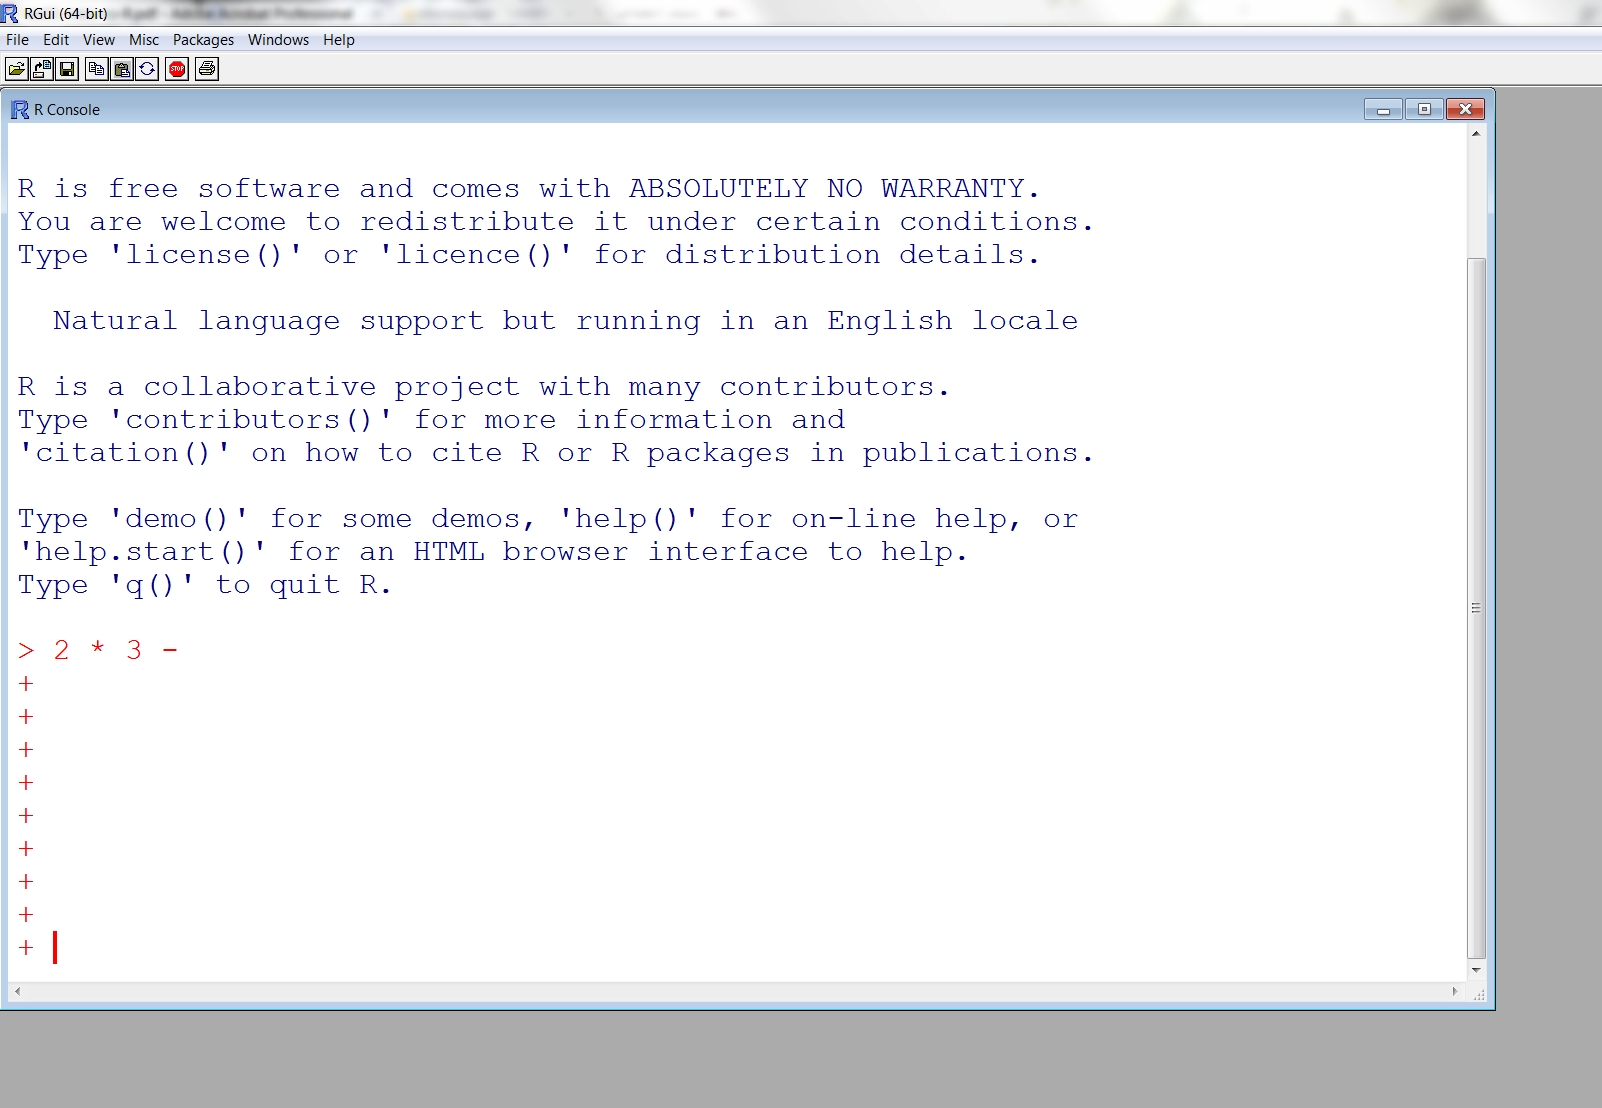
\includegraphics[width=0.7\textwidth]{figs/plus-prompt}
  \end{center}
  \pause
  Just hit the ``Esc'' key or complete the command.
\end{frame}




% NOTE: Make them do this by hand
\begin{frame}[fragile]
  \frametitle{Summarizing vectors}
  \small
  \begin{center}
    \begin{tabular}{ccccc}
      \hline
%      & \multicolumn{5}{c}{Number of chiggers on 5 different people} \\
      \multicolumn{5}{c}{Number of ticks on 5 dogs} \\
      \hline %\cline{1-5}
      $y_1$ & $y_2$ & $y_3$ & $y_4$ & $y_5$ \\
      \hline
      4 & 7 & 2 & 3 & 150 \\
      \hline
    \end{tabular}
  \end{center}
%\begin{itemize}
%\item
What is the sum of this vector? $\sum_{i=1}^5 y_i$ = ???
  \pause
\begin{knitrout}\footnotesize
\definecolor{shadecolor}{rgb}{0.878, 0.918, 0.933}\color{fgcolor}\begin{kframe}
\begin{alltt}
\hlstd{y} \hlkwb{<-} \hlkwd{c}\hlstd{(}\hlnum{4}\hlstd{,}\hlnum{7}\hlstd{,}\hlnum{2}\hlstd{,}\hlnum{3}\hlstd{,}\hlnum{150}\hlstd{)}
\hlkwd{sum}\hlstd{(y)}
\end{alltt}
\begin{verbatim}
## [1] 166
\end{verbatim}
\end{kframe}
\end{knitrout}
\pause
%\item \large
What is the mean? $\frac{\sum_{i=1}^5 y_i}{5}$ = ???
  \pause
\begin{knitrout}\footnotesize
\definecolor{shadecolor}{rgb}{0.878, 0.918, 0.933}\color{fgcolor}\begin{kframe}
\begin{alltt}
\hlkwd{mean}\hlstd{(y)}
\end{alltt}
\begin{verbatim}
## [1] 33.2
\end{verbatim}
\end{kframe}
\end{knitrout}
  \pause
%\item
  And the variance? $\frac{\sum_{i=1}^5 (y_i - \bar{y})^2}{5-1}$ = ???
\begin{knitrout}\footnotesize
\definecolor{shadecolor}{rgb}{0.878, 0.918, 0.933}\color{fgcolor}\begin{kframe}
\begin{alltt}
\hlkwd{var}\hlstd{(y)}
\end{alltt}
\begin{verbatim}
## [1] 4266.7
\end{verbatim}
\end{kframe}
\end{knitrout}
%\end{itemize}
\end{frame}


%\end{document}


%\subsection{Indexing}


\begin{frame}[fragile]
  \frametitle{Indexing vectors}
%  \begin{itemize}[<+->]
%  \item
  \small
  Extract the first and third elements of a vector
\begin{knitrout}\small
\definecolor{shadecolor}{rgb}{0.878, 0.918, 0.933}\color{fgcolor}\begin{kframe}
\begin{alltt}
\hlstd{y} \hlkwb{<-} \hlkwd{c}\hlstd{(}\hlnum{2}\hlstd{,} \hlnum{4}\hlstd{,} \hlnum{8}\hlstd{,} \hlnum{4}\hlstd{,} \hlnum{25}\hlstd{)}
\hlstd{y.sub1} \hlkwb{<-} \hlstd{y[}\hlkwd{c}\hlstd{(}\hlnum{1}\hlstd{,}\hlnum{3}\hlstd{)]}
\hlstd{y.sub1}
\end{alltt}
\begin{verbatim}
## [1] 2 8
\end{verbatim}
\end{kframe}
\end{knitrout}
%\item
\pause \vfill
Remove the second element
\begin{knitrout}\small
\definecolor{shadecolor}{rgb}{0.878, 0.918, 0.933}\color{fgcolor}\begin{kframe}
\begin{alltt}
\hlstd{y.sub2} \hlkwb{<-} \hlstd{y[}\hlopt{-}\hlnum{2}\hlstd{]}
\hlstd{y.sub2}
\end{alltt}
\begin{verbatim}
## [1]  2  8  4 25
\end{verbatim}
\end{kframe}
\end{knitrout}
\pause \vfill
%\item
Rearrange the order of the vector
\begin{knitrout}\small
\definecolor{shadecolor}{rgb}{0.878, 0.918, 0.933}\color{fgcolor}\begin{kframe}
\begin{alltt}
\hlstd{y.re} \hlkwb{<-} \hlstd{y[}\hlkwd{c}\hlstd{(}\hlnum{5}\hlstd{,}\hlnum{4}\hlstd{,}\hlnum{3}\hlstd{,}\hlnum{2}\hlstd{,}\hlnum{1}\hlstd{)]}
\hlstd{y.re}
\end{alltt}
\begin{verbatim}
## [1] 25  4  8  4  2
\end{verbatim}
\end{kframe}
\end{knitrout}
%\end{itemize}
\end{frame}


\begin{frame}[fragile]
  \frametitle{Indexing vectors}
%\begin{itemize}[<+->]
%  \item
  \small
  Which elements of the vector are greater than 4? (logical test)
\begin{knitrout}\small
\definecolor{shadecolor}{rgb}{0.878, 0.918, 0.933}\color{fgcolor}\begin{kframe}
\begin{alltt}
\hlstd{y} \hlkwb{<-} \hlkwd{c}\hlstd{(}\hlnum{2}\hlstd{,} \hlnum{4}\hlstd{,} \hlnum{6}\hlstd{,} \hlnum{4}\hlstd{,} \hlnum{25}\hlstd{)}
\hlstd{y}\hlopt{>}\hlnum{4}
\end{alltt}
\begin{verbatim}
## [1] FALSE FALSE  TRUE FALSE  TRUE
\end{verbatim}
\end{kframe}
\end{knitrout}
\pause \vfill
  Extract the elements greater than 4 (logical indexing)
\begin{knitrout}\small
\definecolor{shadecolor}{rgb}{0.878, 0.918, 0.933}\color{fgcolor}\begin{kframe}
\begin{alltt}
\hlstd{y.sub4} \hlkwb{<-} \hlstd{y[y}\hlopt{>}\hlnum{4}\hlstd{]}
\hlstd{y.sub4}
\end{alltt}
\begin{verbatim}
## [1]  6 25
\end{verbatim}
\end{kframe}
\end{knitrout}
\end{frame}


\subsection{Data frames}


\begin{frame}[fragile]
  \frametitle{Data frames}
  \large
%  \begin{itemize}[<+->]
%    \item
  Most basic datasets are stored as \verb+data.frame+s
  \pause \vfill
%    \item
  They are like a matrix in which each column can be a
      different type of vector (numeric, factor, etc...)
%    \item
  \pause \vfill
   They have attributes for row names (e.g. the names of
      the experimental units) and column names (e.g. the names of
      the response and predictor variables)
%  \end{itemize}
\end{frame}



\begin{frame}[fragile]
  \frametitle{Creating a data frame}
  {Simple example with 3 variables measured at 4 sites}
\begin{knitrout}\small
\definecolor{shadecolor}{rgb}{0.878, 0.918, 0.933}\color{fgcolor}\begin{kframe}
\begin{alltt}
\hlstd{y} \hlkwb{<-} \hlkwd{c}\hlstd{(}\hlnum{3}\hlstd{,} \hlnum{9}\hlstd{,} \hlnum{7}\hlstd{,} \hlnum{4}\hlstd{)}
\hlstd{x1} \hlkwb{<-} \hlkwd{factor}\hlstd{(}\hlkwd{c}\hlstd{(}\hlstr{'High'}\hlstd{,} \hlstr{'High'}\hlstd{,} \hlstr{'Low'}\hlstd{,} \hlstr{'Low'}\hlstd{))}
\hlstd{x2} \hlkwb{<-} \hlkwd{c}\hlstd{(}\hlnum{2.2}\hlstd{,} \hlnum{3.4}\hlstd{,} \hlnum{4.4}\hlstd{,} \hlnum{3.9}\hlstd{)}
\hlstd{mydata} \hlkwb{<-} \hlkwd{data.frame}\hlstd{(}\hlkwc{Goats}\hlstd{=y,} \hlkwc{Elev}\hlstd{=x1,} \hlkwc{Temp}\hlstd{=x2)}
\hlkwd{rownames}\hlstd{(mydata)} \hlkwb{<-} \hlkwd{c}\hlstd{(}\hlstr{'Site1'}\hlstd{,} \hlstr{'Site2'}\hlstd{,} \hlstr{'Site3'}\hlstd{,} \hlstr{'Site4'}\hlstd{)}
\hlstd{mydata}
\end{alltt}
\begin{verbatim}
##       Goats Elev Temp
## Site1     3 High  2.2
## Site2     9 High  3.4
## Site3     7  Low  4.4
## Site4     4  Low  3.9
\end{verbatim}
\end{kframe}
\end{knitrout}
\end{frame}


\begin{frame}[fragile]
  \frametitle{Indexing data frames}
%  \begin{itemize}[<+->]
%    \item
  \small
  Bracket method. Extract data from row 1, columns 1 and 3
\begin{knitrout}\footnotesize
\definecolor{shadecolor}{rgb}{0.878, 0.918, 0.933}\color{fgcolor}\begin{kframe}
\begin{alltt}
\hlstd{mydata[}\hlnum{1}\hlstd{,}\hlkwd{c}\hlstd{(}\hlnum{1}\hlstd{,}\hlnum{3}\hlstd{)]}
\end{alltt}
\begin{verbatim}
##       Goats Temp
## Site1     3  2.2
\end{verbatim}
\end{kframe}
\end{knitrout}
%    \item
\pause \vfill
Bracket method. Extract from rows 2 and 3, columns 1 and 3
\begin{knitrout}\footnotesize
\definecolor{shadecolor}{rgb}{0.878, 0.918, 0.933}\color{fgcolor}\begin{kframe}
\begin{alltt}
\hlstd{mydata[}\hlkwd{c}\hlstd{(}\hlstr{'Site2'}\hlstd{,} \hlstr{'Site3'}\hlstd{),} \hlkwd{c}\hlstd{(}\hlstr{'Goats'}\hlstd{,} \hlstr{'Temp'}\hlstd{)]}
\end{alltt}
\begin{verbatim}
##       Goats Temp
## Site2     9  3.4
## Site3     7  4.4
\end{verbatim}
\end{kframe}
\end{knitrout}
%    \item
\pause \vfill
Dollar sign method. Pull out column 1
\begin{knitrout}\footnotesize
\definecolor{shadecolor}{rgb}{0.878, 0.918, 0.933}\color{fgcolor}\begin{kframe}
\begin{alltt}
\hlstd{mydata}\hlopt{$}\hlstd{Elev}
\end{alltt}
\begin{verbatim}
## [1] High High Low  Low 
## Levels: High Low
\end{verbatim}
\end{kframe}
\end{knitrout}
%  \end{itemize}
\end{frame}


\begin{frame}[fragile]
  \frametitle{Summarizing data frames}
%  \begin{itemize}[<+->]
%    \item
  \small
  View the data as a `spreadsheet'
\begin{knitrout}\footnotesize
\definecolor{shadecolor}{rgb}{0.878, 0.918, 0.933}\color{fgcolor}\begin{kframe}
\begin{alltt}
\hlkwd{View}\hlstd{(mydata)}
\end{alltt}
\end{kframe}
\end{knitrout}
%    \item
\pause \vfill
Compute some summary statistics
\begin{knitrout}\scriptsize
\definecolor{shadecolor}{rgb}{0.878, 0.918, 0.933}\color{fgcolor}\begin{kframe}
\begin{alltt}
\hlkwd{summary}\hlstd{(mydata)}
\end{alltt}
\begin{verbatim}
##      Goats        Elev        Temp      
##  Min.   :3.00   High:2   Min.   :2.200  
##  1st Qu.:3.75   Low :2   1st Qu.:3.100  
##  Median :5.50            Median :3.650  
##  Mean   :5.75            Mean   :3.475  
##  3rd Qu.:7.50            3rd Qu.:4.025  
##  Max.   :9.00            Max.   :4.400
\end{verbatim}
\end{kframe}
\end{knitrout}
%    \item
\pause \vfill
A very compact summary
\begin{knitrout}\scriptsize
\definecolor{shadecolor}{rgb}{0.878, 0.918, 0.933}\color{fgcolor}\begin{kframe}
\begin{alltt}
\hlkwd{str}\hlstd{(mydata)}
\end{alltt}
\begin{verbatim}
## 'data.frame':	4 obs. of  3 variables:
##  $ Goats: num  3 9 7 4
##  $ Elev : Factor w/ 2 levels "High","Low": 1 1 2 2
##  $ Temp : num  2.2 3.4 4.4 3.9
\end{verbatim}
\end{kframe}
\end{knitrout}
%  \end{itemize}
\end{frame}



\subsection{Importing and Exporting Data}

\begin{frame}[fragile]
  \frametitle{Importing and exporting data}
  \verb+read.csv+ and \verb+write.csv+ are easy options, but there are
  many more possibilities that we won't cover. \\
%  \begin{itemize}
%    \item
  \small
  \pause \vfill
  Export the \verb+data.frame+ we created earlier
\begin{knitrout}\small
\definecolor{shadecolor}{rgb}{0.878, 0.918, 0.933}\color{fgcolor}\begin{kframe}
\begin{alltt}
\hlkwd{write.csv}\hlstd{(mydata,} \hlkwc{file}\hlstd{=}\hlstr{"mydata.csv"}\hlstd{)}
\end{alltt}
\end{kframe}
\end{knitrout}
%    \item
  \pause \vfill
Confirm that it is there:
\begin{knitrout}\scriptsize
\definecolor{shadecolor}{rgb}{0.878, 0.918, 0.933}\color{fgcolor}\begin{kframe}
\begin{alltt}
\hlkwd{getwd}\hlstd{()} \hlcom{# Go to this location and look for 'mydata.csv'}
\end{alltt}
\end{kframe}
\end{knitrout}
%    \item
  \pause \vfill
Read it back in:
\begin{knitrout}\small
\definecolor{shadecolor}{rgb}{0.878, 0.918, 0.933}\color{fgcolor}\begin{kframe}
\begin{alltt}
\hlstd{mydata2} \hlkwb{<-} \hlkwd{read.csv}\hlstd{(}\hlstr{"mydata.csv"}\hlstd{)}
\end{alltt}
\end{kframe}
\end{knitrout}
%  \end{itemize}
\end{frame}







\begin{frame}[fragile]
  \frametitle{The working directory}
The working directory is the location on your computer where \R~will
look for files by default. \\
\pause \vfill
You can check your working directory like this:
\begin{knitrout}\small
\definecolor{shadecolor}{rgb}{0.878, 0.918, 0.933}\color{fgcolor}\begin{kframe}
\begin{alltt}
\hlkwd{getwd}\hlstd{()}
\end{alltt}
\begin{verbatim}
## [1] "c:/Work/exp-design/labs/intro-to-R"
\end{verbatim}
\end{kframe}
\end{knitrout}
\pause \vfill
Change your working directory to another location:
\begin{knitrout}\small
\definecolor{shadecolor}{rgb}{0.878, 0.918, 0.933}\color{fgcolor}\begin{kframe}
\begin{alltt}
\hlcom{## Note the forward slashes, which could be replaced by "\textbackslash{}\textbackslash{}"}
\hlkwd{setwd}\hlstd{(}\hlstr{"C:/work/courses/"}\hlstd{)}
\end{alltt}
\end{kframe}
\end{knitrout}
\pause \vfill
\centering
{\bf At the beginning of every \R~session, you should use
  \inr{setwd} to set your working directory \\}
\end{frame}








\subsection{Removing objects and saving workspaces}

\begin{frame}[fragile]
  \frametitle{The workspace}
%  \begin{itemize}[<+->]
%    \item
  Viewing the objects in your workspace
\begin{knitrout}\scriptsize
\definecolor{shadecolor}{rgb}{0.878, 0.918, 0.933}\color{fgcolor}\begin{kframe}
\begin{alltt}
\hlkwd{ls}\hlstd{()}
\end{alltt}
\begin{verbatim}
##  [1] "BMI"      "clean"    "filestub" "height"   "mydata"   "mydata2" 
##  [7] "open"     "reqval"   "rnw.file" "tangle"   "weight"   "x1"      
## [13] "x2"       "y"        "y.re"     "y.sub1"   "y.sub2"   "y.sub4"  
## [19] "y1"       "y2"       "z"
\end{verbatim}
\end{kframe}
\end{knitrout}
%    \item
\pause \vfill
Removing (deleting) some objects
\begin{knitrout}\scriptsize
\definecolor{shadecolor}{rgb}{0.878, 0.918, 0.933}\color{fgcolor}\begin{kframe}
\begin{alltt}
\hlkwd{rm}\hlstd{(x1, x2, mydata2, y, y1, y2, y.re,}
   \hlstd{y.sub1, y.sub2, y.sub4, height, weight, BMI, z)}
\hlkwd{ls}\hlstd{()}
\end{alltt}
\begin{verbatim}
## [1] "clean"    "filestub" "mydata"   "open"     "reqval"   "rnw.file"
## [7] "tangle"
\end{verbatim}
\end{kframe}
\end{knitrout}
%  \end{itemize}
\end{frame}





\begin{frame}[fragile]
  \frametitle{Saving and restoring the workspace}
  \begin{center}
    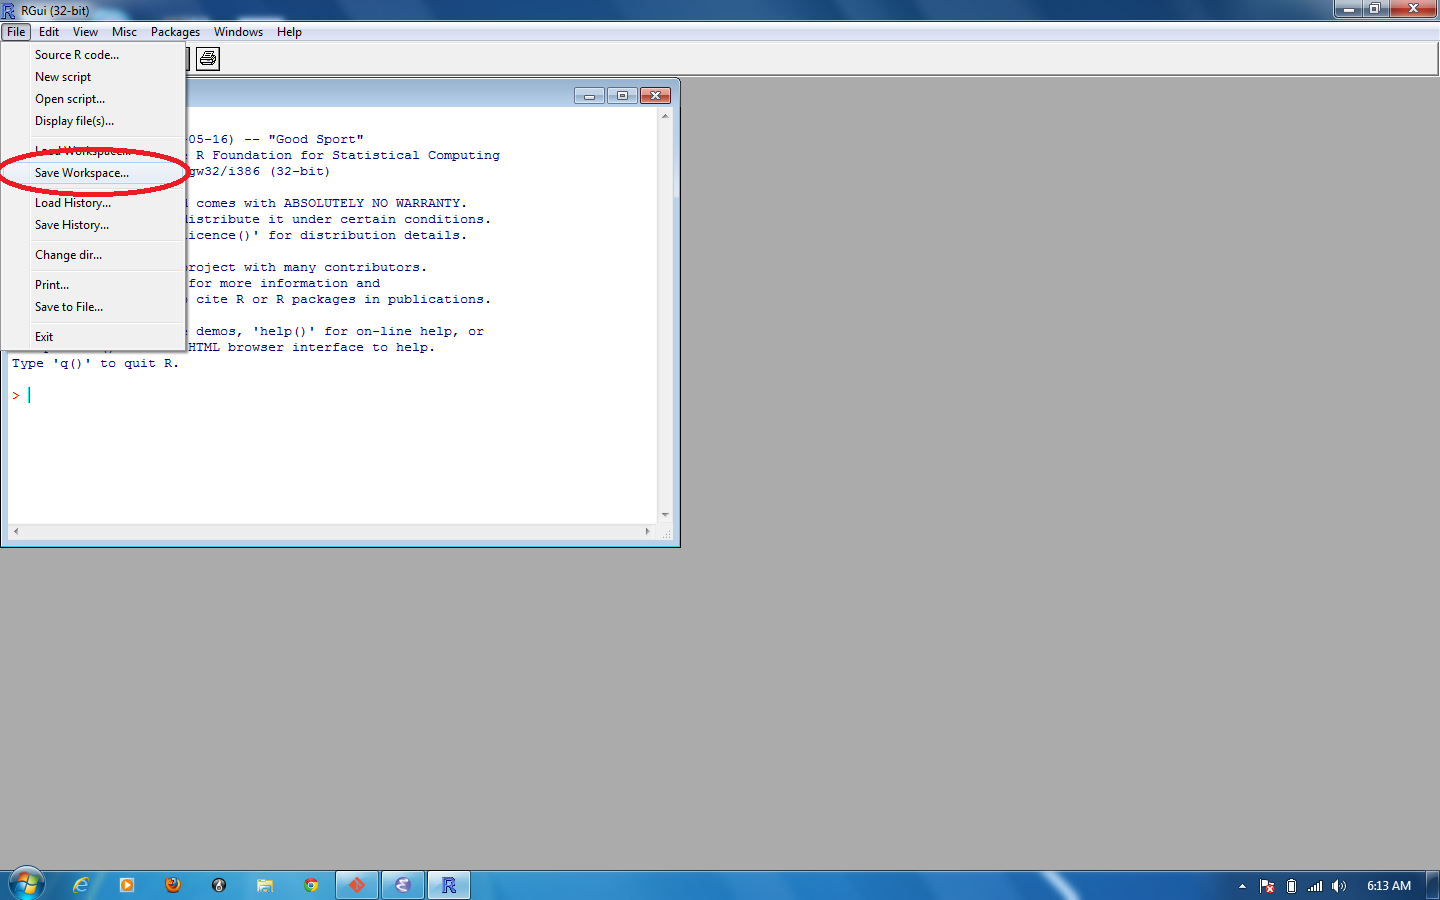
\includegraphics[width=0.8\textwidth]{figs/save-workspace}
  \end{center}
  \pause
If you prefer commands over point-and-click:
\begin{knitrout}
\definecolor{shadecolor}{rgb}{0.878, 0.918, 0.933}\color{fgcolor}\begin{kframe}
\begin{alltt}
\hlkwd{save.image}\hlstd{(}\hlstr{"myimage.RData"}\hlstd{)} \hlcom{# Save all objects to file}
\hlkwd{load}\hlstd{(}\hlstr{"myimage.RData"}\hlstd{)}       \hlcom{# Load the saved workspace}
\end{alltt}
\end{kframe}
\end{knitrout}
\end{frame}




\section{Getting help}



\begin{frame}[fragile]
  \frametitle{Additional Resources}
  \large
%\begin{itemize}
%  \item
  `Official' manuals
\begin{knitrout}
\definecolor{shadecolor}{rgb}{0.878, 0.918, 0.933}\color{fgcolor}\begin{kframe}
\begin{alltt}
\hlkwd{help.start}\hlstd{()}
\end{alltt}
\end{kframe}
\end{knitrout}
%  \item[]
%  \item
\vfill
Useful books
\begin{itemize}
  \large
\item Venables, W.N. and B.D. Ripley. 2002. Modern Applied Statistics with
  S, 4th ed. Springer.
\item Crawley, M.J.. 2013. The \R~Book, 2nd ed. Wiley
\end{itemize}
%  \item[]
%  \item
\vfill
Online
    \begin{itemize}
      \large
      \item Always Google your error messages
      \item \url{http://stackoverflow.com/}
      \item \url{https://preludeinr.com/}
    \end{itemize}
%\end{itemize}
\end{frame}






\begin{frame}[fragile]
  \frametitle{Assignment -- Part I}
  \footnotesize
  \begin{enumerate}[\bf (1)]
    \item Create an \R~script named something like \verb+Chandler-R_lab1.R+
    \item In your \R~script, write code to create a \verb+data.frame+
      that contains the information shown in the table below
    \item Add code to export the \verb+data.frame+ as a .csv file and
      then import it back into \R.
  \end{enumerate}
  \begin{center}
    \scriptsize
    \begin{tabular}{lccc}
      \hline
      Individual & Mass & Weight & Treatment \\
      \hline
      1 & 3 & 4 & Control \\
      2 & 3 & 5 & Control \\
      3 & 2 & 4 & Control \\
      4 & 4 & 6 & Treatment \\
      5 & 5 & 5 & Treatment \\
      6 & 5 & 7 & Treatment \\
      \hline
    \end{tabular}
  \end{center}
  Upload your \R~script\footnote{\scriptsize \noindent If you
    are familiar with RMarkdown, you can submit a \texttt{.Rmd} file
    instead of a \texttt{.R} file} to ELC before your next lab. The script should
  be self-contained, meaning that it will run correctly when we copy
  and paste it in the console.
\end{frame}



\begin{frame}[fragile]
  \frametitle{Assignment -- Part II}
  \begin{columns}
    \begin{column}{0.3\textwidth}
      
\includegraphics[width=1\textwidth]{figs/introStatsR} \\
%      \tiny
    \end{column}
    \begin{column}{0.6\textwidth}
%      \begin{enumerate}[\bf (1)]
%        \item
      Read chapters 1, 4, \& 5 before next lab
%        \item[]
%        \item Create an R script to import a .csv file (you can use
%          any file you want). Upload the script and the .csv file to
%          ELC.
%      \end{enumerate}
    \end{column}
  \end{columns}
  \vfill
  \footnotesize
  Dalgaard, P. 2008. Introductory Statistics with R. 2nd
  edition. Springer. \\
%  \vspace{0.3cm}
  Available for free through the UGA library: \\ \tiny
  \url{http://preproxy.galib.uga.edu/login?url=http://dx.doi.org/10.1007/978-0-387-79054-1}
\end{frame}



\end{document}
